\pagestyle{fancy}
\fancyhead[R]{Física Nuclear y de Partículas: Tema 3}
\fancyhead[L]{4º Grado en Física}
\chapter{El núcleo atómico. Propiedades Globales}
Los núcleos atómicos son complicados de estudiar. Su característica más general es que están formados por \textbf{nucleones}, ésto nos genera el primer problema y es que \textbf{no} tenemos un nucleón privilegiado sobre el que podamos establecer un origen sobre el que realicemos transformaciones.
\section{Generalidades del núcleo}
El núcleo atómico es un sistema muy complejo (muchas partículas), sobre el que tenemos que considerar las 3 interacciones fundamentales: electromagnética fuerte y débil. Por ser un sistema de muchos cuerpos, los estudios se realizan desde un punto de vista fenomenológico.\\\\
Los núcleos por están compuestos por nucleones $(p,n)$ podemos definir tres números: $A$, número másico; $Z$, número atómico; $N=A-Z$, número de neutrones. Podemos establecer así diferentes relaciones entre núcleos:\\\\
\noindent
\begin{minipage}{0.4\textwidth}
    \begin{itemize}
    \item Si tienen \textbf{misma} $Z$ se conocen como isótopos.
    \item Si tienen \textbf{misma} $N$ se conocen como isótonos.
    \item Si tienen \textbf{misma} $A$ se conocen como isóbaros.
\end{itemize}
\end{minipage}
\hfill
\begin{minipage}{0.55\textwidth}
    \begin{tcolorbox}[colback=amber!20, colframe=amber, title={Notación: Representación de los núcleos}]
    Los núcleos los vamos a representar através de su símbolo químico $X$ y índices, $A$ como superíndice y $Z$ como subíndice a la izquierda, a veces representaremos $N$ como un subíndice a la derecha.
    \begin{equation}
        ^A_ZX_N
    \end{equation}
\end{tcolorbox}
\end{minipage}\\\\

Se conocen nucleos con número másico $A=1,290$ y unos 2000 núcleos distintos de los quales $\sim250$ son estables y $\sim350$ quasi-estables.

\subsubsection{Estabilidad nuclear}
Otra clasificación que podemos hacer es en función del número de partículas que componen el núcleo, si nos centramos en los núcleos estables encontramos
\newpage

\begin{table}[h]
\centering
\begin{tabular}{c|ccc|}
\cline{2-4}
 & \multicolumn{1}{c|}{Z} & \multicolumn{1}{c|}{N} & \begin{tabular}[c]{@{}c@{}}nº de núcleos \\ estables\end{tabular} \\ \hline
\multicolumn{1}{|c|}{\multirow{2}{*}{A=impar}} & Impar & Par   & $50$  \\
\multicolumn{1}{|c|}{}                         & Par   & Impar & $55$  \\ \cline{1-1}
\multicolumn{1}{|c|}{\multirow{2}{*}{A=par}}   & Par   & Par   & $165$ \\
\multicolumn{1}{|c|}{}                         & Impar & Impar & $4$   \\ \hline
\end{tabular}
\caption{Número de núcleos estables en función del número de nucleones que lo componen. Los núlceos pares tipo $(I,I)$  sólo son 4 y son núcleos ligeros: $^2_1 \mathrm{H},\  ^6_3 \mathrm{Li}, \ ^{10}_5 \mathrm{B}, \  ^{14}_7 \mathrm{N}$.}
\label{tab: nucleos estables en funcion del numero de nucleones}
\end{table}

Si recordamos la figura \ref{fig: Diagrama Segre}, para $A<40, Z\approx N$ tenemos que los núcleos son simétricos, mientras que a partir de $A\sim 40$, el cociente $N/Z$ va aumentando hasta tomar valores de 1.54 (uránidos).\\\\
Existen valores de $Z$ y $N$ denominados \textbf{números mágicos} para los que hay un elevado número de núcleos estables : 2, 8, 20, 28, 50, 82, 126. A partir de $Z>83$ no tenemos núcleos estables ya que se desintegran por emisión de partículas $\alpha$ (núcleos de $^4\mathrm{He}$), el núcleo estable de mayor $Z$ es el $^{209}_{\ 83}\mathrm{Bi}$.\\\\
Los núcleos atómicos pueden tener en lugar de un nucleón un barión $\Delta$, lo que se conoce como \textbf{hipernúcleos}, así tenemos isótopos como el $^{\ \ 6}_{\Lambda \Lambda}\mathrm{He}$ constituído por $^{\ \ 6}_{\Lambda \Lambda}\mathrm{He}=2p+2n+2\Lambda$, estos núcleos no son estables en la superficie de la Tierra, pero pueden existir en situaciones extremas como cortezas de estrellas de neutrones.

\subsubsection{Sistema de muchas partículas}
Debido a que el núcleo es un sistema de muchas partículas, tenemos un número de grados de libertad demasiado grande como para poder considerarlos todos, por ello utilizaremos un conjunto de observablaes a los que denominamos \textbf{propiedades estáticas del núcleo}: Carga eléctrica, radio nuclear, masa nuclear, energía de ligadura, momento angular, paridad, momentos electromagnéticos...

\section{Distribución de carga y masa nuclear. Factores de forma}

El tamaño y la forma de un objeto se analizan a partir de la radiación que dispersan, para ello necesitamos que la longitud de onda de la radiación \footnote{No tiene que ser necesariamente radiación electromagnética, recordar que existe la longitud Compton\\ $\lambda_\mathrm{C}=\dfrac{h}{p}$}con la que estamos bombardenado el objeto sea $\lambda \lesssim $ tamaño del objeto. Así podemos determinar las distribuciones de carga y masa:
\begin{itemize}
    \item \textbf{Distribución carga nuclear}: se determina mediante un scattering del núcleo con electrones, y permiten determinar la estructura interna (protones y neutrones) del núcleo. La razón por la que se utilizan leptones se debe a que ellos \textbf{no} participan en la interacción fuerte.
    \item \textbf{Distribución de masa nuclear}: se determina a partir de un scattering Rutherford, para ello se utilizan partículas $\alpha=2p+2n$ a muy alta energía, esto hace que podamos romper el scattering Rutherford y entre en juego la fuerza fuerte, lo que nos permite ver el tamaño del núcleo.
\end{itemize}
\subsection{Distribución de carga nuclear}
Si recordamos de la figura \ref{tab: comparacion de escalas}, el radio nuclear es de $r_\mathrm{N}\sim \unit[10]{fm}$, por lo que la longitud de onda que deben tener los electrones con los que bombardeemos el núcleo será $$\lambda \lesssim \unit[10]{fm} \Rightarrow p>\dfrac{h}{\lambda}=\dfrac{2\pi \hbar c}{pc}\sim \unit[100]{MeV/\textit{c}^2}$$

Por lo que estamos utilizando electrones \textbf{ultrarrelativistas} $(pc\gg mc^2)$. Este tratamiento nos permite realizar un tratamiento ondulatorio del electrón, si suponemos que el núcleo es un disco esférico de diámetro $D$, nos aparece como no podía ser de otra manera un patrón de Airy que toma por expresión en el primer mínimo:
\begin{equation}
    \sin\theta=1.22\frac{D}{\lambda}
    \label{Difraccion de Airy}
\end{equation}
    \begin{tcolorbox}[colback=airforceblue!20, colframe=airforceblue, title={Ejemplo: Patrones de difracción del $^{12}\mathrm{C}$ y $^{16}\mathrm{O}$.}]
Si incidimos con un haz de electrones con una energía de $\unit[420]{MeV}$ sobre un núcleo de $^{12}\mathrm{C}$ encontramos que el primer mínimo se encuentra a 51,5\degree, así podemos obtener el tamaño del núcleo $$\lambda=\frac{2\pi \hbar c}{pc}\Rightarrow D=\frac{1.22}{\sin(51.5\degree)} \frac{2\pi 197.327}{420}=\unit[4.6]{fm}$$
Por lo que el radio del $^{12}\mathrm{C}, r(^{12}\mathrm{C})=\unit[2.3]{fm}$, del mismo modo si incidimos con un haz con la misma energía sobre $^{16}\mathrm{O}$ encontramos que el primer mínimo de difracción está en 43.8\degree lo que nos da un radio de $r(^{16}\mathrm{O})=\unit[2.6]{fm}$.\\\\
Así mismo si cambiamos la energía del haz incidente a $\unit[360]{MeV}$ para el oxígeno-16, encontramos el mínimo en $53.9\degree$ que nos da el mismo radio.
\end{tcolorbox}

\noindent \begin{minipage}{0.6\textwidth}
    Si realizamos un scattering sobre núcleos pesados, observamos que hay varios mínimos de difracción a diferentes ángulos pero ninguno se hace nulo (figura \ref{fig:Scattering de electrones y nucleos}), este comportamiento se debe a que el núcleo no es rígido como una bola de billar, sino que es difuso al estilo de la nube electrónica de un átomo (figura \ref{fig: Distribucion de carga nuclear}).\\\\
De la figura \ref{fig: Distribucion de carga nuclear} podemos extraer que la densidad de carga del núcleo es aproximadamente igual en el centro independientemente de $A$. A medida que nos alejamos del centro la densidad de carga empieza a caer de manera progresiva, así definimos \textit{skin thickness} ($t$) como la distancia en la que la densidad de carga pasa de valer el 90\% de su valor central al 10\%.
\end{minipage}
\hfill
\begin{minipage}{0.35\textwidth}
    \centering
    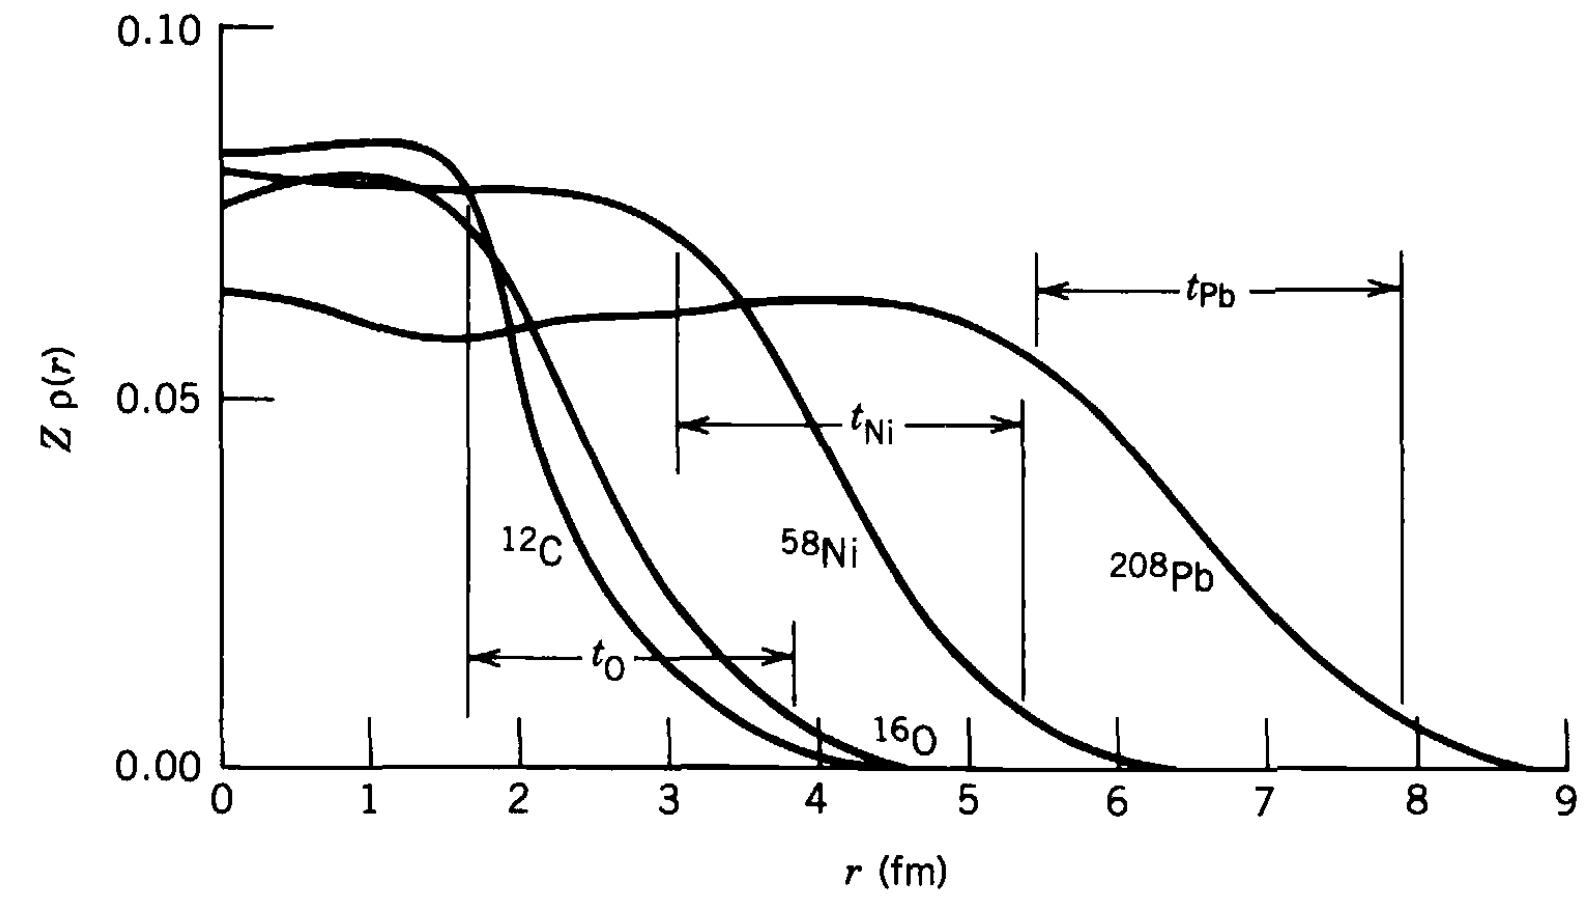
\includegraphics[width=\linewidth]{Diagramas Tema 3/Densidad de carga nucleos.png}
    \captionof{figure}{Distribución de carga de distintos núcleos en función del radio.}
    \label{fig: Distribucion de carga nuclear}    
\end{minipage}

\noindent
\begin{minipage}{0.55\textwidth}
Una cantidad de gran importancia para la física nuclear es la sección eficaz de un scattering elástico de electrones con una carga puntual (scattering $e^-+e^+$). En un scattering relativista tenemos que la sección eficaz diferencial viene dada por 
\begin{equation}
    \eval{\dv{\sigma}{\Omega}}_\mathrm{Mott}=\frac{\alpha^{2}Z^{2}(\hbar c)^{2}}{4E^{2}v^{4}\sin^{4}\left(\frac{\theta}{2}\right)}\left[1-\frac{v^{2}}{c^{2}}\sin^{2}\left(\frac{\theta}{2}\right)\right]
    \label{eq: seccion eficaz mott}
\end{equation}

Que es la versión relativista del scattering Rutherford. Ahora bien, si cambiamos la carga puntual por un núcleo, simplemente tenemos que introducir el \textbf{factor de forma}\footnotemark.
\begin{equation}
    \eval{\dv{\sigma}{\Omega}}_\mathrm{Exp}=\eval{\dv{\sigma}{\Omega}}_\mathrm{Mott}\abs{F(q)}^2
\end{equation}
\end{minipage}
\footnotetext{El desarrollo del factor de forma y del radio cuadrático medio lo encontramos en el apéndice \ref{chap: Apendice C}.}
\hfill
\begin{minipage}{0.4\textwidth}
    \centering
    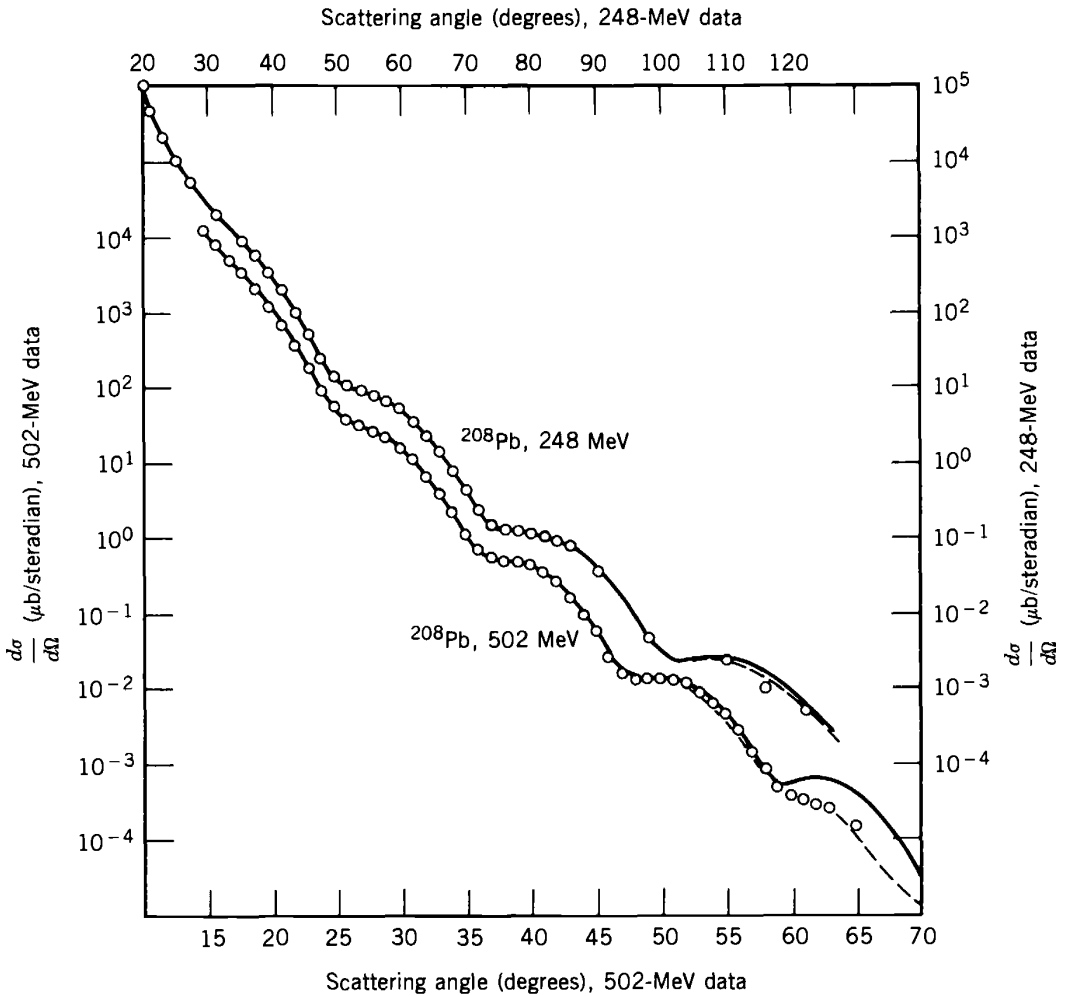
\includegraphics[scale=0.25]{Diagramas Tema 3/Scattering de Plomo.png}
    \captionof{figure}{Scattering de electrones sobre núcleos de $^{208}\mathrm{Pb}$.}
    \label{fig:Scattering de electrones y nucleos}
\end{minipage}
\\\\

Así podemos hacer predicciones postulando la distribución de carga y calculando su factor de forma podemos ver cómo se amolda a los datos experimentales\footnote{El proceso inverso es imposible realizarlo ya que no es posible alcanzar todos los datos numéricos necesarios para realizar al integral impropia de la transformada.}. Volviendo al análisis que hicimos de la figura \ref{fig: Distribucion de carga nuclear} podemos determinar el radio nuclear 
\begin{equation}
 \frac{A}{\frac{4}{3}\pi R^3}=\text{cte} \Rightarrow R=R_0A^{1/3} \quad \text{con} \quad R_0=\unit[1.23]{fm}
    \label{eq: radio nuclear}
\end{equation}

\noindent Mientras que para la \textit{skin thickness} tenemos que el valor es $t\approx \unit[2.3]{fm}$.
\\\\
La distribución que mejor reproduce estos resultados es la distribución de Fermi
\begin{equation}
    \rho(r)=\dfrac{\rho_0}{1+\exp{\dfrac{r-c}{a_0}}}
    \label{eq: distribucion de Fermi}
\end{equation}
Donde $c$ es la disntancia donde $\rho(c)=\dfrac{1}{2} \rho_0$, y $a_0$ es un parámetro empírico que nos dice cómo decae la distribución, que para núcleos con $A\ge 20$ tenemos que 
\begin{equation*}
    c=\unit[1.07 A^{1/3}]{fm} \quad \quad \quad a_0=\unit[0.54]{fm}\equiv \text{cte}
\end{equation*}
\subsubsection{Radio equivalente de una distribución de carga uniforme}
Si calculamos el radio cuadrático $\expval{r^2}=\displaystyle  \dfrac{\int_0^\infty r^4 \rho \dd r}{\int_0^\infty r^2 \rho \dd r}=\dfrac{3}{5}R^2$, así $\expval{r^2}^{1/2}=\sqrt{\frac{3}{5}}R\approx \unit[0.94 A^{1/3}]{fm}$. Obtenemos el radio equivalente de una distribución uniforme, lo que es más fácil de integrar y no se aleja demasiado de los resultados experimentales.
\newpage

\subsubsection{Métodos alternativos}
El análisis de las distribuciones de carga lo podemos hacer a partir de transiciones atómicas, para ello hacemos uso de los potenciales
\begin{equation}
    V_\mathrm{Puntual}(r)=-\frac{Ze^2}{4\pi \varepsilon_0 r} \quad \quad V_\mathrm{Extenso}(r)= \left \{
\begin{aligned}
& \quad\frac{-Ze^2}{4\pi\varepsilon_0R}\left\{\frac{3}{2}-\frac{1}{2}{\left(\frac{r}{R}\right)}^2\right\} \quad \text{si} \quad r\le R \\\\
& \quad\frac{-Ze^2}{4\pi\varepsilon_0r} \quad \text{si} \quad r\ge R
\end{aligned} \right.
\label{eq: potenciales de transicion atomica}
\end{equation}

Si utilizamos que la transiciones más probables son aquellas que siguen la regla de selección $\Delta \ell =1$, tenemos que la función de onda del orbital más interno es $\Psi(r)=\displaystyle \sqrt{\frac{Z^3}{\pi a_0^3}}\exp{-\frac{Zr}{a_0}}$ con lo que la diferencia de energía entre núcleos puntuales y extenso es es 
\begin{equation}
    \Delta E=\expval{V}_\mathrm{Extenso}-\expval{V}_\mathrm{Puntual}=\frac{2}{5} \frac{Z^4e^2}{4\pi\varepsilon_0}\frac{R^2}{a_0^3}
\end{equation}
Para transiciones $K_\alpha (2p \xrightarrow{} 1s)$ encontramos que el incremento de energía en isótopos vecinos es
\begin{equation*}
    E_K(A)-E_K(A^{\prime})=-\frac{2}{5}\frac{Z^4e^2}{4\pi\varepsilon_0}\frac{R_0^2}{a_0^3}{\left(A^{2/3}-{A^{\prime }}^{2/3}\right)}
\end{equation*}

Esto nos permite hacer un ajuste obteniendo que $R_0=\unit[1.2]{fm}$ como no podía ser de otra manera.\\\\
La ventaja de utilizar este método es que nos permite estudiar los núcleos de $Z$ elevado, ya que si cambiamos un electrón por un muón el radio de Bohr $(a_0^\mu(\mathrm{^{208}Pb})=\unit[3]{fm})$ se reduce considerablemente y encontramos que el muón puede estar dentro del núcleo ya que $R=\unit[7.1]{fm}$.
\subsection{Distribución de masa nuclear}
Hasta ahora hemos utilizado únicamente el scattering de leptones con protones, pero queremos saber la relevancia que tienen los neutrones dentro del mismo.\\\\
Como ya hemos mencionado, para estudiar esta distribución utilizamos partículas $\alpha$ y en función de la energía cinética que tengan las partículas podemos determinar la influencia de la interacción fuerte.\\\\
De la misma manera que utilizamos muones para estudiar el núcleo atómico, podemos utilizar piones ya que estos participan en la interacción fuerte. Comparando los rayos X emitidos por un átomo piónico con los calculados usando sólo la interacción coulombiana obtenemos información acerca de la extensión del núcleo. Por último como la absorción de los piones por parte de los nucleones no emite rayos X se genera un defecto que también puede ser medible.
\newpage
\section{Spín, paridad y momentos electromagnéticos nucleares}
Como ya sabemos, el núcleo es un sistema formado por $A$ cuerpos, pero el hamiltoniano que describe este sistema $H= \displaystyle \sum_i^A -\dfrac{\hbar^2}{2m_i} \laplacian-V(\vec{r}_1,\cdots, \vec{r}_A)$ no es posible resolverlo de manera exacta. Sin embargo el simple hecho de que se pueda escribir nos dice que podemos tener estados ligados (espectro discreto de energía), además la función de onda que describa los estados del núcleo debe ser completamente antisimétrica, por último sabemos que los estados excitados se desintegran emitiendo radiación electromagnética.

\subsection{Spín nuclear}

Definimos el momento angular de un núcleo como la suma de los momentos angulares de spin $s_i$ y momentos angulares orbitales $l_i$
\begin{equation}
    \vec{J}=\sum_i^A \vec{l}_i+\vec{s}_i=\sum_i^A \vec{j}_i
\end{equation}

Como le potencial no tiene por qué ser central no podemos utilizar el momento angular orbital como número cuántico pero sí que podemos utilizar el total, tomando los operadores $J_z$ y $J^2$ para la base de autofunciones los valores esperados son $\expval{J_z}=\hbar m$ con $m=-J,\cdots, J$ y $ \expval{J^2}=J\hbar^2(J+1)$.
\\\\
\noindent Tenemos varias restricciones sobre los momentos angulares totales de los nucleones:
\begin{itemize}
    \item Por ser fermiones, los nucleones tienen $j_i$ semientero, por lo que si $A$ es par, $J$ es un entero mientras que si $A$ es impart $J$ es semientero.
    \item Experimentalmente se ha medido que para los nucleos con $(Z,N)=$ (par,par) el estado fundamental es $J=0$. El $J$ de un núcleo con $A$ semientero, se puede entender en muchas ocasiones en términos del spin del nucleón desapareado.
\end{itemize}

\noindent Al hecho de que en el estado fundamental de los núcleos con $A$ par $J=0$ se le conoce como \textbf{pairing}, esto confiere estabilidad a los núcleos ya que los acoplamientos de spin sólo se dan en partículas idénticas, es decir, $(p,p)$ y $(n,n)$ ya que son los únicos casos en los que podemos tener acoplamiento a spin total $J=0,1$.

\subsection{Paridad nuclear}
Como la paridad es una simetría de la interacción fuerte y de la interacción electromagnética, debe ser un buen número cuántico para los estados nucleares. Como vemos en la figura \ref{fig:espectro de energia y JP de los nucleos}, los estados están identificados por $J^P$ y dentro de un núcleo podemos tener distintos estados excitados.
\newpage
\begin{figure}[h]
    \centering
    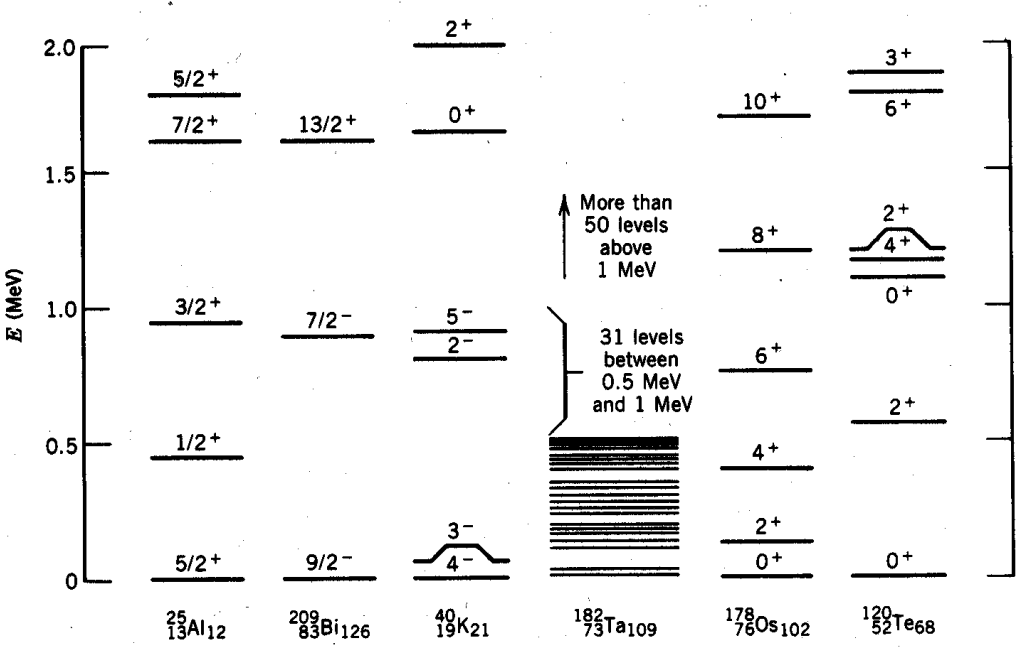
\includegraphics[width=0.7\linewidth]{Diagramas Tema 3/Espectro de energía de distintos nucleos.png}
    \caption{Espectro de energía de diferentes núcleos atómicos. Se muestran además la $J^P$ los diferentes estados de los núcleos.}
    \label{fig:espectro de energia y JP de los nucleos}
\end{figure}

La paridad de los nucleones por convenio está fijada a $P_N =+$ mientras que para los antinucleones será $P_{\Bar{N}} =-$. La paridad del núcleo la podemos calcular entonces como\\ $P=(-)^L\prod_i^A P_i$, pero como no podemos conocer los diferentes momentos angulares orbitales, tomaremos la paridad del nucleón como un dato experimental que \textbf{no} tiene relación teórica con el momento angular total $J$ del núcleo.
\\\\
Experimentalmente se ha medido que para los núcleos (par,par) tienen $J^P=0^+$, además como pasaba para los núcleos con $A$ impar la paridad la podemos determinar en muchas ocasiones en función del nucleón desapareado.
\subsection{Momento dipolar magnético}

El momento dipolar magnético nos permite estudiar la dinámica de un sistema en el seno de un campo magnético. El momento magnético de un sistema lo podemos calcular como 
\begin{equation}
    \vec{\mu}=\sum_i^A \vec{\mu}_i=\frac{1}{\hbar}\qty(g_i^{(l)}\vec{l}_i+ g_i^{(s)}\vec{s}_i)\frac{e \hbar c }{2m_p c} \quad \text{con} \quad g_i^{(l)}=\left \{ \begin{aligned}
        &g_p^{(l)}=1 \\
        &g_n^{(l)}=0
    \end{aligned} \right., \quad g_i^{(s)}=\left \{ \begin{aligned}
        &g_p^{(s)}=5.58 \\
        &g_n^{(s)}=-3.82
    \end{aligned} \right.
    \label{eq: momento magnetico}
\end{equation}

Donde los $g_i$ son las razones giromagnéticos en términos del magnetón nuclear $\mu_N=\dfrac{e \hbar c}{2m_p c}$. Debido a las fuerzas de pairing y a la expresión \ref{eq: momento magnetico} sólo contribuyen al momento magnético los nucleones desapareados (siempre podemos descomponer un núcleo en un corazón (par,par)+(0,1) ó (1,0)). Esta propiedad nos permite tratar los núcleos como partículas únicas ya que únicamente con la partícula desapareada y su spin, obtenemos todas las propiedades del núcleo.\\\\

\subsection{Momento cuadrupolar eléctrico}
El momento cuadrupolar eléctrico lo medimos en barn [$\unit[1]{b}=\unit[10^{-26}]{m^2}$] y su valor está entre $[-1,8]$b. El momento cuadrupolar eléctrico se define como
\begin{equation}
    Q_{20}=e\sqrt{\frac{16\pi}{5}}\langle\psi(\vec{r})|r^2\mathrm{Y}_{20}^*(\theta,\varphi)|\psi(\vec{r})\rangle=e\langle J,J|3z^2-r^2|J,J\rangle=e\left[3\langle z^2\rangle-\langle r^2\rangle\right]
    \label{eq: momento cuadrupolar}
\end{equation}
\noindent
\begin{minipage}{0.6\textwidth}
    y nos da información sobre la forma que tiene el núcleo:
\begin{itemize}
    \item Si $\langle z^2\rangle=\langle x^2\rangle=\langle y^2\rangle\to Q_{20}=0\Rightarrow$ El núcleo es esférico.
    \item Si $\langle z^2\rangle>\langle x^2\rangle=\langle y^2\rangle\to Q_{20}>0\Rightarrow$ El núcleo es prolato.
    \item Si $\langle z^2\rangle<\langle x^2\rangle=\langle y^2\rangle\to Q_{20}<0\Rightarrow$ El núcleo es oblato.
\end{itemize}

En el momento cuadrupolar nuclear tenemos contribución de todos los nucleones salvo en las proximidades de los números mágicos, esto es similar al caso de los gases nobles cuya contribución cuadrupolar es 0 debido a que todos los electrones que tienen están en capa cerrada.\\\\
En la figura \ref{fig: momentos quadrupolares} observamos que los núcleos en las proximidades de algunos números hacen su momento cuadrupolar nulo (muy bajo), a estos números de nucleones se les conocen como \textbf{números mágicos}. Esto parece sugerir que en el núcleo tenemos una estructura de capas.
\end{minipage}
\hfill
\begin{minipage}{0.35\textwidth}
    \centering
    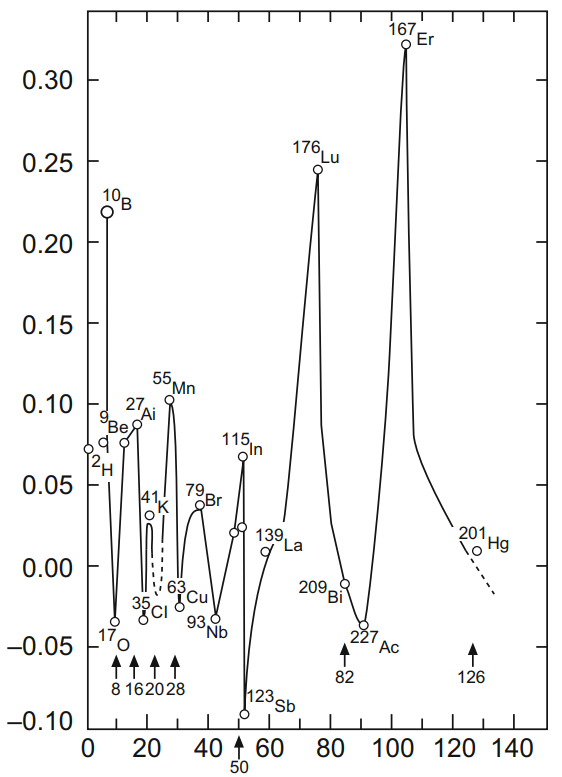
\includegraphics[width=\linewidth]{Diagramas Tema 3/Momentos cuadrupolares de los nucleos.png}
    \captionof{figure}{Momentos cuadrupolares reducidos para núcleos con número impar de protones \( Z \) o neutrones \( N \) graficados en función de este número.}
    \label{fig: momentos quadrupolares}
\end{minipage}

\section{Masa de los núcleos. Fórmula semiempírica de masas} 
Vamos a definir la masa de un núcleo como 
\begin{equation}
    M_\mathrm{nucleo}c^2=m(^A_Z X_N)c^2-Zm_ec^2+\sum_{i=1}^Z  
 B_i^e
 \label{eq: masa de un nucleo}
\end{equation}
donde $m(^A_Z X_N)$ es la masa del átomo (no del núcleo) y $B_i^e$ es la energía de ligadura que siente cada uno de los electrones, este término es despreciable ya que estas energía son del orden de los rayos X $(\unit[10-100]{keV})$ y la masa de un nucleón es del orden de los GeV.
\subsection{Energías de ligadura y de separación}
De manera análoga para el caso de los átomos, la energía de ligadura de un núcleo la definimos como 
\begin{equation}
    B(^A_Z X_N)=\qty[Z m(^1\mathrm{H})+Nm_n- m(^A_Z X_N)]c^2
    \label{eq: energia de ligadura}
\end{equation}

\begin{tcolorbox}[colback=applegreen!20, colframe=applegreen, title={Definición: Unidad de masa atómica}]
    Definimos la unidad de masa atómica como 
    \begin{equation*}
        \unit[1]{uma}=\frac{m\qty(^{12}\mathrm{C})}{12}
    \end{equation*}
\end{tcolorbox}

Podemos expresar la unidad de masa atómica en MeV, resultando $\unit[1]{uma}=\unit[931.5]{MeV}$, es decir, dentro del núcleo los nucleones son más ligeros por la energía de ligadura.\\\\
Definimos la energía de ligadura por nucleón como $\dfrac{B}{A}$ y el defecto de masa de un núcleo como 
\begin{equation}
    ^A \Delta = m(^A_Z X_N)c^2-\unit[A]{[uma]}
    \label{eq: defecto de masa}
\end{equation}

\begin{figure}[h]
        \centering
    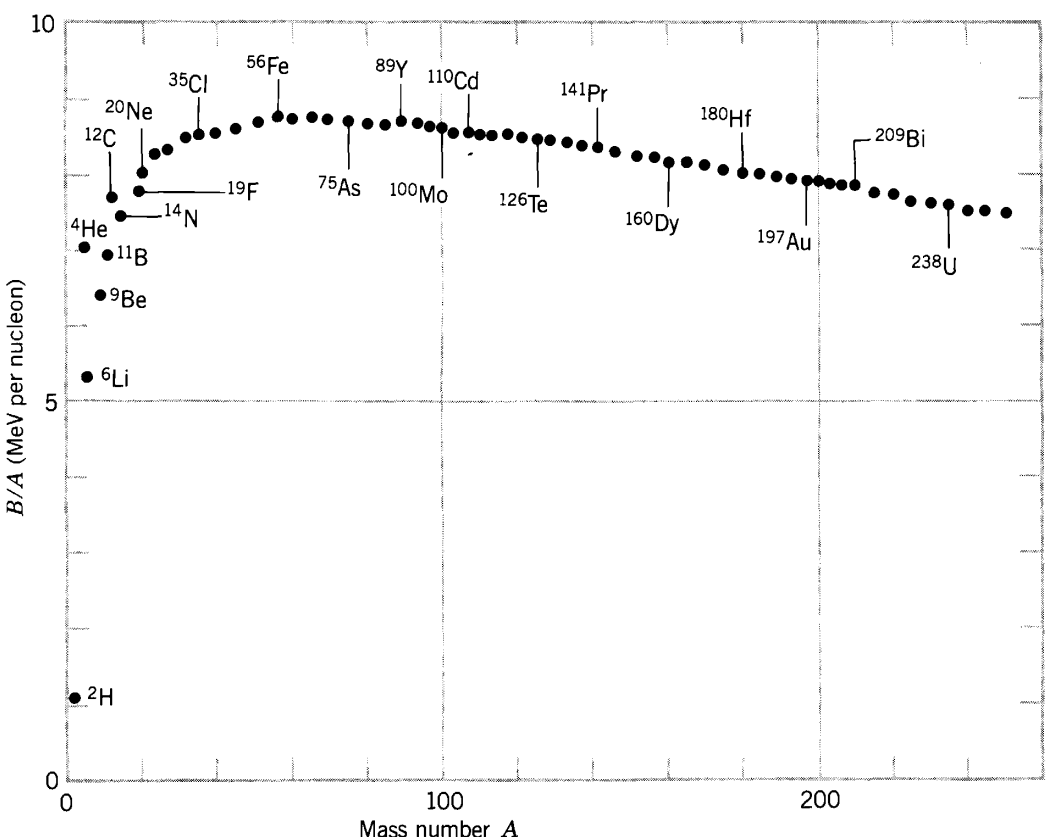
\includegraphics[width=\linewidth]{Diagramas Tema 3/Energia de ligadura por nucleon.png}
    \caption{Energía de ligadrua por nucleón en función del número de nucleones. Como vemos el núcleo de carbono-12 está fuera de la curva, al igual que las el núcleo de $^4$He (partícula $\alpha$).}
    \label{fig: energia de ligadura por nucleon frente al numero masico}
\end{figure}

Podemos utilizar el defecto de masa para saber cómo es la robustez del núcleo atómico, si el núcleo tiene mayor defecto de masa el núcleo estará más ligado que el átomo de $^{12}$C y viceversa
    $$\left \{ \begin{aligned}
        &^A \Delta >0 \xrightarrow[]{} \frac{B}{A}(^A_Z X_N)< \frac{B}{A}(^A_Z \mathrm{C})\\
        &^A \Delta <0 \xrightarrow[]{} \frac{B}{A}(^A_Z X_N)> \frac{B}{A}(^A_Z \mathrm{C})
    \end{aligned}   \right.$$

Si analizamos la figura \ref{fig: energia de ligadura por nucleon frente al numero masico} la energía es más o menos constante $\nicefrac{B}{A}\sim \unit[8]{MeV}$ salvo para núcleos ligeros. Esta curva tiene un máximo en $A\approx 60$, por lo que los núcleos atómicos que tienden a llegar a  este estado liberan energía de dos maneras
\begin{itemize}
    \item Para $A<60$ la energía de enlace por nucleón aumenta cuando añadimos nucleones, lo que conocemos como \textbf{fusión}.
    \item Para $A>60$ Aumentamos la energía de ligadura fraccionando los núcleos, lo que conocemos como \textbf{fisión}.
\end{itemize}

    Otra energía que podemos definir es la energía de separación, que es la energía que tenemos que darle a un núcleo para arrancarle un protón o un neutron.
    \begin{equation}
        \left \{  \begin{aligned}
    & S_n=\qty[m\qty(^{A-1}_Z X_{N-1})+m_n-m(^A_Z X_N)]c^2=B\qty(^A_Z X_N)-B\qty(^{A-1}_Z X_{N-1})\\
    &S_p=\qty[m\qty(^{A-1}_{Z-1} X_{N})+m\qty(^1\mathrm{H})-m(^A_Z X_N)]c^2=B\qty(^A_Z X_N)-B\qty(^{A-1}_{Z-1} X_{N})
        \end{aligned}
        \right.
        \label{eq: energías de separacion para el neutron y el proton}
    \end{equation}
    Este concepto es análogo a las energías de ionización en un átomo.\\
    \begin{tcolorbox}[colback=airforceblue!20, colframe=airforceblue, title={Ejemplo: Fusión del Deuterio en Helio-4}]
    Dada la siguiente reacción
    \begin{equation*}
        ^2\mathrm{H}+^2\mathrm{H} \longrightarrow ^4\mathrm{He}
    \end{equation*}
    Si hacemos uso de la ecuación \ref{eq: masa de un nucleo} y comparamos las energías de ambos miembros de la reacción, para el primer miembro tenemos  $2\qty(m_p+m_n-B_{^2\mathrm{H}})$ mientras que en el segundo $2m_p+2m_n-B_{^4\mathrm{He}}$, como las masas de los nucleones contribuyen de igual manera, la energía obtenida de la reacción es la diferencia de las energías de ligadura, como $\unit[B_{^2\mathrm{H}}=4.4]{MeV}$ y $\unit[B_{^4\mathrm{He}}=28]{MeV}$ obtenemos $\unit[24]{MeV}$ de la reacción.
\end{tcolorbox}

\subsection{Fórmula semiempírica de masas (Weizsäcker)}

Para intentar reproducir la curva que aparece en la figura \ref{fig: energia de ligadura por nucleon frente al numero masico} vamos a introducir la fórmula semiempírica de masas, esta fórmula no es reproducible por ningún (único) modelo nuclear. .\\\\

En lo primero que tenemos que pensar es cómo interaccionan los nucleones dentro del núcleo, volviendo a la figura \ref{fig: energia de ligadura por nucleon frente al numero masico}, vemos que a partir de $A=15$ la energía por nucleón varía entre $ \unit[[7.4,8.8]]{MeV}$, es decir, no es exactamente constante (como sí lo sería si todos los nucleones interaccionasen con todos) por lo que diremos que la interacción nuclear \textbf{satura}. 
\\\\
Veamos los términos que ha de tener la fórmula semiempírica de masas:
\begin{itemize}
    \item \textbf{Término de volumen} $a_\mathrm{V}A$: Como la interacción nuclear satura, la densidad del núcleo es \textbf{constante}, esto implica que cada nucleón tiene el mismo número de vecinos y cada nucleón contribuye a $B$ con la misma intensidad. Como hemos dicho que la densidad es constante y el núcleo es más o menos esférico, el volumen va como $R^3=R_0^3A$ la energía debe seer proporcional a $A$.
    \item \textbf{Término de superficie} $a_\mathrm{S}A^{2/3}$: Los nucleones que se encuentran en la superficie no tienen el mismo número de vecinos que los que se encuentran dentro del núcleo por lo que están menos ligados. Esta contribución resta (ya que estaríamos contando de más), y de manera análoga al término de volumen, la superficie de la esfera va como $R^2=R_o^2A^{2/3}$, este término ha de ser proporcional a $A^{2/3}$.
    \item \textbf{Término de Coulomb} $a_\mathrm{C}Z(Z-1)A^{-1/3}$: Los protones se repelen entre sí debido a la fuerza de Coulomb. Si hay $Z$ protones todos se repelen entre sí, luego el término es proporcional a $Z(Z-1)$. Si asumimos que la distribución de la carga es uniforme:
    \begin{equation}
        E_\mathrm{C}=-\frac{3}{5} \frac{e^2}{4\pi\varepsilon_0} \frac{Z(Z-1)}{R}=-\frac{3}{5} \frac{e^2}{4\pi\varepsilon_0} \frac{Z(Z-1)}{R_0A^{1/3}}
    \end{equation}
    Este término también resta (ya que separa los nucleones) y es proporcional a $Z(Z-1)A^{-1/3}$.
    \item \textbf{Término de simetría} $a_\mathrm{sym}\dfrac{(A-2Z)^2}{A}$: En la figura \ref{fig: Diagrama Segre} (plot de Segre) los núcleos con $A<40$ son simétricos, es decir, $N\approx Z \approx \nicefrac{A}{2}$. Por encima de este valor $\nicefrac{Z}{A}\approx \nicefrac{1}{2}$. Por lo que este término es cero si $Z=\nicefrac{A}{2}$ y su importancia decrece con $A$.\\\\
    Este término tiene gran relevancia en los núcleos pesados, pues de no existir tendríamos núcleos con un número infinito de neutrones.
    \item \textbf{Término de apareamiento} $\delta$: Tiene en cuenta la tendencia observada de los nucleones a agruparse por parejas. Si $A$ es impar el término no contribuye. Si $A$ es par tenemos dos posibilidades:
    \begin{itemize}
        \item Si $Z$ y $N$ son impares $B$ aumentará al transformar un neutrón en un protón o viceversa.
        \item Si $Z$ y $N$ disminuye $B$ al transformar un nucleón en otro.
    \end{itemize}
    Podemos parametrizarlo mediante la siguiente función \footnote{El exponente también puede ser $-\nicefrac{3}{4}$}
    \begin{equation}
        \delta = \left \{ \begin{aligned}
            &- a_\mathrm{p}A^{-1/2}  & \quad \text{si} \quad \text{(I,I)}\\
            &0 & \quad \text{si} \quad \text{(I,P) ó (P,I)} \\
            & a_\mathrm{p}A^{-1/2} & \quad \text{si} \quad \text{(P,P)}
        \end{aligned} \right.
    \end{equation}
    \label{eq: termino de pairing}
\end{itemize} 

Así la fórmula semiempírica de masas será
\begin{equation}
    \begin{aligned}
        &m(^A_Z X_N)c^2=\qty[Z m(^1\mathrm{H})+Nm_n]c^2-B(^A_Z X_N) \quad \mathrm{con} \\
        &B(^A_Z X_N)=a_\mathrm{V}A-a_\mathrm{S}A^{2/3}-a_\mathrm{C}\frac{Z(Z-1)}{A^{1/3}}-a_\mathrm{sym} \frac{(A-2Z)^2}{A}+\delta(A)
    \end{aligned}
    \label{eq: formulas semiempirica de masas}
\end{equation}


Fijémonos que esta ecuación \textbf{no considera los números mágicos}, por lo que en sus proximidades observaremos fluctuaciones.\\\\
La fórmula semiempírica de masas incorpora características individuales y globales de los núcleos, los 3 primeros términos considera al núcleo un ente global (partícula única), mientras que los 2 últimos hemos utilizado propiedades de los constituyentes (nucleones).

\begin{table}[h]
\centering
\begin{tabular}{|ccccc|}
\hline
\multicolumn{1}{|c|}{$a_\mathrm{V}$} &
  \multicolumn{1}{c|}{$a_\mathrm{S}$} &
  \multicolumn{1}{c|}{$a_\mathrm{C}$} &
  \multicolumn{1}{c|}{$a_\mathrm{sym}$} &
  $a_\mathrm{p}$ \\ \hline \hline
$\unit[15.67]{MeV}$ &
  $\unit[17.23]{MeV}$ &
  $\unit[0.72]{MeV}$ &
  $\unit[23.287]{MeV}$ &
  $\unit[12 \footnotemark]{MeV}$ \\ \hline
\end{tabular}
\caption{Valor de las constantes de la fórmula semiempírica de masas.}
\label{tab: constantes de Formula semiempirica de masas}
\end{table}
\footnotetext{En el caso de utilizar el exponente $-\nicefrac{3}{4}$, el valor de esta constante es $a_\mathrm{p}=\unit[34]{MeV}$}
\section{Inestabilidad nuclear}
La fórmula semiempírica de masas nos permite analizar la estabilidad de los núcleos, así como en qué modos va hacia la estabilidad. Si tenemos una reacción $$a+A\longrightarrow b+B$$
Definimos el \textbf{factor \textit{Q}} como 
\begin{equation}
    Q=\qty[M(a)+M(A)-M(b)-M(B)]c^2 \left \{ \begin{aligned}
        &Q>0 \quad \text{Exotérmica}\\
        &Q<0 \quad \text{Endotérmica}
    \end{aligned} \right.
    \label{eq: factor Q}
\end{equation}
Para el caso de las desintegraciones, la reacción tiene la forma $A\xrightarrow[]{} b+c+\cdots$ y para que se produzcan de manera espontánea $Q>0$
\subsection{Tipos de desintegraciones radiactivas} \label{sec: Tipos de desintegraciones radiactivas}
\begin{itemize}
    \item \textbf{Desintegración $\bm{\alpha}$}: El núcleo emite una partícula $\alpha\equiv\, ^{\ 4}\mathrm{He}$. La desintegración tiene la forma 
    \begin{equation*}
        ^A _Z X_N \longrightarrow ^{A-4} _{Z-2} Y_{N-2}+ ^4\mathrm{He}
    \end{equation*}
        
    Como vimos en el apéndice \ref{chap: Apendice B}, por ser una desintegración a dos cuerpos (no relativista + relativista) con la energía de las partículas $\alpha$ está \textbf{discretizada}.
    \item \textbf{Desintegración $\bm{\beta^-}$}: El núcleo corrige el exceso de neutrones transformando un neutrón en un protón y emitiendo el electrón resultante junto con un antineutrino
    \begin{equation*}
        ^A _Z X_N \longrightarrow ^{\ \ \ A} _{Z+1} Y_{N-1}+ e^-+\Bar{\nu}_e
    \end{equation*}

        Por ser una desintegración a tres cuerpos (2 relativistas + 1 pesado) el electrón presenta un espectro continuo de energías.

    \item \textbf{Desintegración $\bm{\beta^+}$}:  El núcleo corrige el exceso de protones transformando un neutrón en un protón y emitiendo el positrón resultante junto con un neutrino
    \begin{equation*}
        ^A _Z X_N \longrightarrow ^{\ \ \ A} _{Z-1} Y_{N+1}+ e^++{\nu}_e
    \end{equation*}

    De igual menera, el positrón presenta un espectro contínuo de energías \ref{fig: Emisioones electrones}

    \item \textbf{Captura electrónica}: El núcleo corrige un exceso de protones absorbiendo un electrón atómico y emitiendo el neutrino correspondiente
    \begin{equation*}
        ^A _Z X_N +e^- \longrightarrow ^{\ \ \ A} _{Z-1} Y_{N+1}++{\nu}_e
    \end{equation*}

    Esto compite con la desintegración $\beta^+$, pero sólo en los casos en los que tenemos $M_X-M_Y<2m_e$ ya que si no se cumpliese no se conserva la energía y estaría prohibido.

    \item \textbf{Desintegración $\bm{\gamma}$}: Un núcleo de un estado excitado se desintegra a su estado fundamental emitiendo un fotón 
    $${^A _Z X_N }^*\longrightarrow ^A _Z X_N+\gamma$$
    
    El espectro de los fotones emitidos es \textbf{discreto}.
    
    \item \textbf{Conversión interna}: El núcleo en un estado excitado se desintegra a su estado fundamental transfiriendo energía a un electrón atómico que es expulsado.
    $${^A _Z X_N }^*\longrightarrow ^A _Z X_N+e^-$$

    Esta desintegración compite con la desintegración $\gamma$, y el espectro de los electrones emitidos es discreto, los electrones al reordenarse emiten rayos X con energías discretas.
    \item \textbf{Fisión espontánea}: Un núcleo pesado se fragmenta en dos núcleos más ligeros
    $${^A _Z X_N }^*\longrightarrow {^{A^\prime} _{Z^\prime} Y_{N^\prime}+ ^{A-A^\prime} _{Z-Z^\prime} Y_{N-N^\prime}  }$$
    La distribución de la masa de los núcleos resultantes sigue una  distribución asimétrica, por ejemplo, en la desintegración del $^{235} _{92} \mathrm{U} \longrightarrow ^{95}\mathrm{Kr}+^{137}\mathrm{Ba}$
    \item \textbf{Emisión de un nucleón}: Un nucleón expulsa el exceso de nucleones. Suele darse tras una fisión nuclear y es cómo se originan las reacciones en cadena en un reactor.
\end{itemize}

\section{Parábolas de estabilidad}
La fórmula semiempírica de masas \ref{eq: formulas semiempirica de masas} la podemos escribir como una parábola:
\begin{equation}
    M(A,Z)=\gamma Z^2-\beta Z + \alpha \quad \text{con} \quad \left \{ 
    \begin{aligned}
    &\gamma= \frac{a_\mathrm{C}}{A^{1/3}}+4\frac{a_\mathrm{sym}}{A} \\
    &\beta=-m_pc^2+m_nc^2-4a_\mathrm{sym}\qty(\frac{a_\mathrm{C}}{A^{1/3}}) \\
    &\alpha= m_nc^2-a_\mathrm{V} +a_\mathrm{S}A^{-1/3}+a_\mathrm{sym} + \frac{\delta}{A}
    \end{aligned} \right.
\end{equation}

Si fijamos $A$ y minimizamos la función $M(A,Z)$, obtenemos el elemento químico más estable para un $A$ dado.
\begin{equation}
    Z^\mathrm{Th}_\mathrm{min}=\frac{(m_n-m_p)c^2+4a_\mathrm{sym}}{2\frac{a_\mathrm{c}}{A^{1/3}}+8\frac{a_\mathrm{sym}}{A}}
    \label{eq: Z minimo para un A constante}
\end{equation}

Esta ecuación si $A$ es pequeño se comporta como $Z^\mathrm{Th}_\mathrm{min} \xrightarrow[]{} A/2$; si $A$ es grande $Z^\mathrm{Th}_\mathrm{min}<A/2$; y para $A$ muy grandes $Z^\mathrm{Th}_\mathrm{min}/A\approx 0.4 $.
\subsubsection{Parábolas de estabilidad. Núcleos impares}
    Los núcleos impares se desplazan sobre la parábola de estabilidad a través de las desintegraciones fundamentales $\textcolor{blue}{\beta^-}$, $\textcolor{applegreen}{\beta^+}$ ó \textcolor{applegreen}{CE}; hasta alcanzar el valor $Z_\mathrm{min}$.
\subsubsection{Parábolas de estabilidad. Núcleos Pares}
    En el caso de los núcleos pares tendreemos dos núcleos estables para un $A$ fijo, uno con vida media infinita (estable) y otro con vida media muy larga, que sólo se podría desintegrar por doble desintegración $\beta$ (línea punteada de la figura \ref{fig: Parabola Estabilidad A par})
\begin{figure}[h]
    \begin{subfigure}{0.45\textwidth}
            \centering
    \includegraphics[width=\linewidth]{Diagramas Tema 3/ParabolaEstabilidadAimpar.pdf}
    \caption{Parábola de estabilidad para $A$ impar.} 
    \label{fig: Parabola Estabilidad A impar}
    \end{subfigure}
    \hfill
    \begin{subfigure}{0.45\textwidth}
            \centering
    \includegraphics[width=\linewidth]{Diagramas Tema 3/ParabolaEstabilidadApar.pdf}
    \caption{Parábolas de estabilidad para $A$ par.} 
    \label{fig: Parabola Estabilidad A par}
    \end{subfigure}
    \caption{Parábolas de estabilidad.}
\end{figure}